%%%%%%%%%%%%%%%%%%%% author.tex %%%%%%%%%%%%%%%%%%%%%%%%%%%%%%%%%%%
%
%% sample root file for your "contribution" to a contributed volume
%
%% Use this file as a template for your own input.
%
%%%%%%%%%%%%%%%% Springer %%%%%%%%%%%%%%%%%%%%%%%%%%%%%%%%%%%%%%%%%
%
%
%%% RECOMMENDED %%%%%%%%%%%%%%%%%%%%%%%%%%%%%%%%%%%%%%%%%%%%%%%%%%%
%\documentclass[graybox]{svmult}
%%
%%% choose options for [] as required from the list
%%% in the Reference Guide
%%
%\usepackage{mathptmx}       % selects Times Roman as basic font
%\usepackage{helvet}         % selects Helvetica as sans-serif font
%\usepackage{courier}        % selects Courier as typewriter font
%%\usepackage{type1cm}        % activate if the above 3 fonts are
                             %% not available on your system
%%
%\usepackage{makeidx}         % allows index generation
%\usepackage{graphicx}        % standard LaTeX graphics tool
%%                             % when including figure files
%\usepackage{multicol}        % used for the two-column index
%\usepackage[bottom]{footmisc}% places footnotes at page bottom
%
%
%\usepackage[colorlinks=true]{hyperref}
%\hypersetup{urlcolor=blue, citecolor=blue}
%
%
%% see the list of further useful packages
%% in the Reference Guide
%
%\makeindex             % used for the subject index
                       %% please use the style svind.ist with
                       %% your makeindex program
%
%%%%%%%%%%%%%%%%%%%%%%%%%%%%%%%%%%%%%%%%%%%%%%%%%%%%%%%%%%%%%%%%%%%%%%%%%%%%%%%%%%%%%%%%%%
%
%\begin{document}

\title{Software systems for global optimization and the applied optimization problems}
\titlerunning{Software systems for global optimization } 

\author{Victor Gergel, Konstantin Barkalov, Alexander Sysoyev }
\authorrunning{V.Gergel, K. Barkalov, A. Sysoyev} 

\institute{Victor Gergel, Konstantin Barkalov, Alexander Sysoyev  \at Lobachevsky State University of Nizhni Novgorod,  Nizhni Novgorod, Russia \email{konstantin.barkalov@itmm.unn.ru}}
%
% Use the package "url.sty" to avoid
% problems with special characters
% used in your e-mail or web address
%
\maketitle

\abstract{This paper contains a description of the program systems for solving global optimization problems which have been developed by the authors. The first two systems -- GlobaLab and ParaLab -- are intended for educational and research goals and allow one to study both the known and new global search algorithms. These systems enable to realize the statement of an optimization problem, to choose a method of its solving, to execute a computational experiment and to analyze the results obtained. Such the capacities allow assimilating an experience in solving various global optimization problems, evaluating their efficiency and getting necessary knowledge and skills. After the study of the theory and practical training in optimization on the base of the abovementioned systems the reader can get acquainted with the GlobalExpert system that provides the possibility of solving complicated optimization problems arising in different areas of applications. The examples of solving the applied problems in the fields of optimal design, chemical research and economics are given.}


\section{The software system GlobaLab for investigation and study of global optimization methods}

Globalizer Laboratory (\textit{GlobaLab}) is an integrated software system for carrying out the experiments with the global search methods for study and investigation of the basic concepts, approaches, and the algorithms in the field of \textbf{global optimization}.

The multiextremal optimization problems considered within the framework of the theory of global search are the subject of extensive studies and are applied widely in computer aided design, in solving the identification problems, etc. GlobaLab belongs to the class of systems for carrying out the computational experiments, the development of which is an important area of the novel research techniques in various fields of science and technologies.

The availability of all necessary tools for carrying out the computational experiments is a distinguishing feature of the system. Using GlobaLab, the user of the system (\textit{the optimizer}) can formulate the statement of an optimization problem, select the optimizing algorithm from the list of the global search methods available in the system, set up the graphic indicators for monitoring the global search process, carry out various computational experiments, obtain and analyze the experiment results. These completeness and orientation on the novel technologies of education distinguish GlobaLab from other systems (such as, for example, SYMOP \cite{7_Gergel1993} and LGO \cite{7_Pinter1996}).

The possible fields of application of the system are:
\begin{itemize}
\item \textit{education}: applying by the students and teachers for their investigations and study of the global search methods within the framework of the laboratory training for various disciplines of the optimization oriented curriculum (optimization methods, system analysis, operations research, etc.). GlobaLab can be used for demonstrations of a number of important concepts of mathematics and computer science (sequences, limit points, convergence of a numerical method, etc.). GlobaLab can also be used as an example of a complex approach to the development of the computer simulation systems;

\item \textit{research}: applying by the researchers in the fields of the multiextremal optimization theory for the investigations of the efficiency of the global search algorithms under development. The system can be used as a tool for preparing and carrying out the scientific demonstrations of numerical solving the optimization problems by various methods;

\item \textit{applications}: applying by the experts and researchers as a training component of the complex professional optimization systems.
\end{itemize}

\begin{figure}[t]
%\sidecaption[t]
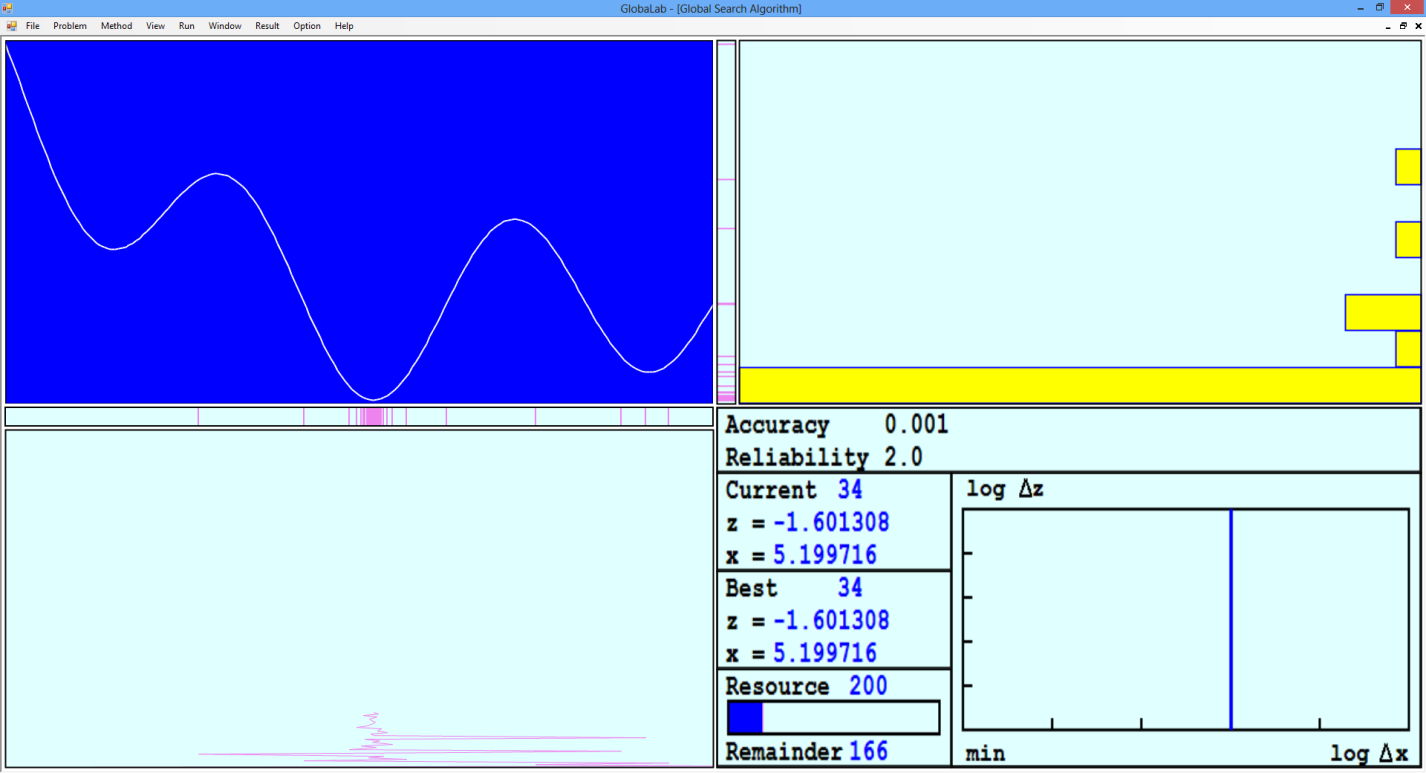
\includegraphics[width=1.0\linewidth]{figures/7_1.png}
\caption{GlobaLab main window}
\label{7_fig_1}     
\end{figure}

The users beginning to study the global search problems can find GlobaLab to be useful to get acquainted with the multiextremal optimization methods. The experienced optimizers can use the system to estimate the efficiencies of newly developed global search algorithms. A screenshot of the GlobaLab main window is presented in Fig.~\ref{7_fig_1}.

\textbf{Capacities of the system.} GlobaLab is an integrated program environment for carrying out the experiments with the global search methods. The user of the system is allowed:

\begin{itemize}
\item \textit{to formulate the statement of the optimization problem}. The minimized function can be selected from a list of the standard functions, generated by a random generator, defined by a formula, or formed by a graphic editor;

\item \textit{to select a global search algorithm} from the list of the optimization methods implemented in the system. GlobaLab supports 10 various multiextremal algorithms, the most known in the theory and practice of the global search. The system provides a possibility to extend the set of methods by the build-in tools without using the algorithmic programming languages;

\item \textit{to set up the graphic indicators} for monitoring the global search process; these indicators allow visualizing the graph of the minimized function or its piecewise linear approximation, the distribution, density, and sequence of the iteration points and of the function values at these points. Monitoring the indicators in the global search process provides better understanding of the global optimization theory and develops the intuition necessary for the practical application and further development of the multiextremal optimization methods;

\item \textit{to carry out various computational experiments} sequentially or in parallel. The latter case allows visual comparing the search dynamics by various methods and is realized in the time sharing mode. Carrying out the series of computational experiments requiring long computation times can be performed automatically with the option of storing the search results for further analysis of the data obtained. Executing the numerical experiments can be performed in the manual mode as well, when the optimizer indicates the iteration points manually (this mode allows the user to verify various hypotheses, which can serve as the base for the development of novel global search methods);

\item \textit{to accumulate and analyze the results of the computational experiments}. GlobaLab allows estimating the operation characteristics of the methods and provides the logging of the experiments in order to record the results of the optimization. The accumulated data can be presented in various generalized forms (tables, graphs, charts) convenient for further analysis. The results of the computations can be stored in a system archive, printed out, or copied to the Windows as text, graphics, or table and transferred to Word, Excel, or another Windows application programs for further processing and analysis (including for the use in preparing the scientific publications, reports, etc.).
\end{itemize}


\section{The software system ParaLab for studying and investigation of the parallel computation methods}

Parallel Laboratory (\textit{ParaLab}) is a software system that provides the possibility to carry out the computational experiments with the purpose of studying and investigation of the parallel algorithms for solving complex computational problems. The system can be used in the laboratory training in various training courses in the field of parallel programming, within which the following possibilities are provided:

\begin{itemize}
\item \textit{the modeling of the parallel multiprocessor computation systems} with different topologies of the networks for the data transfer; 

\item \textit{the visualization} of the computational processes and of the data transfer operations at the parallel solving of different computational problems; 

\item \textit{the estimation of the efficiency} of the parallel computation methods studied.
\end{itemize}

The conduction of such training can be organized on the «ordinary» single processor computers running under the operation systems of MS Windows family (the multiprocess parallel computations simulation mode). Besides the simulation mode, ParaLab can provide the remote access to a multiprocessor computational system for carrying out the numerical experiments in the «true» parallel computations mode in order to compare the results of simulation with the ones of real parallel computations.

In general, ParaLab system is an integrated computational environment for studying and investigation of the parallel algorithms for solving complex computational problems. A wide choice of available tools for the visualization of the computational experiment execution process and for the analysis of the obtained results allows studying the efficiency of application of various algorithms using various computational systems, to make the conclusions on the scalability of the algorithms, and to determine possible speedup for the parallel computation processes.

The educational and research capabilities provided by ParaLab are directed onto the active learning of the theoretical basics and methods, onto encouraging the students to develop their own ideas on the models and methods of the parallel computations by visualization, comparison, and analysis of large set of various graphic indicators and viewers, activated during the experiments.

The main application area of the system is the application in education by the students and teachers for the investigation and studying the parallel algorithms for solving the complex computational problems within the framework of the laboratory practicum in various training courses in the field of parallel programming. ParaLab system can be used also in carrying out research for the estimation of the parallel computations. The users, beginning to study the problems of parallel computing will find ParaLab system to be useful in learning the methods of parallel programming. The experienced programmers can use the system to estimate the efficiency of newly developed parallel algorithms.
A screenshot of the main window of ParaLab system, which a test optimization problem was run in, is presented in Fig.~\ref{7_fig_2}).

\textbf{Capacities of the system.} ParaLab is a software system, which allows conducting the real parallel computations on a multiprocessor computational system as well as the simulations of such experiments on a single serial computer with the visualization of the process of the parallel solving a complex computational problem.

In carrying out the simulation experiments, ParaLab provides the following possibilities for the users:

\begin{itemize}
\item \textit{to define the topology} of the parallel computational system for carrying out the experiments, to define the number of processors in this topology, to set the performance of the processors, to select the parameters of the communication environment and the communication method;

\item \textit{to formulate the statement of the computational problems}, for which in the system there are the built-in parallel algorithms to solve it, to set the parameters of the problem;

\item \textit{to select a parallel method} for solving the specified problem;

\item \textit{to set the visualization parameters} to choose the desired rate of the demonstration, the displaying method for the data transferred between the processors, and the level of the visualization details in the parallel computations;

\item \textit{to carry out the computational experiments} on the parallel solving the specified problem; several different \textit{computational experiments} can be formed in ParaLab with different types of multiprocessor systems, problems, or parallel methods, which the experiments can be run in parallel (in the time sharing mode); the parallel execution of several experiments allows to compare the dynamics of the problem solving by various methods using various topologies with various parameters of the studied problem. If a series of experiments is executed requiring long-time computations, the system provides a possibility to execute the experiments in an automatic mode with saving the numerical results for further analysis of the obtained data,

\item \textit{to accumulate and analyze the results of the experiments}; the system provides the tools for visualizing the saved data featuring the parallel computations (computation time, speedup, efficiency) as the functions of the parameters of the problem and of the computational system.
\end{itemize}

\begin{figure}[t]
%\sidecaption[t]
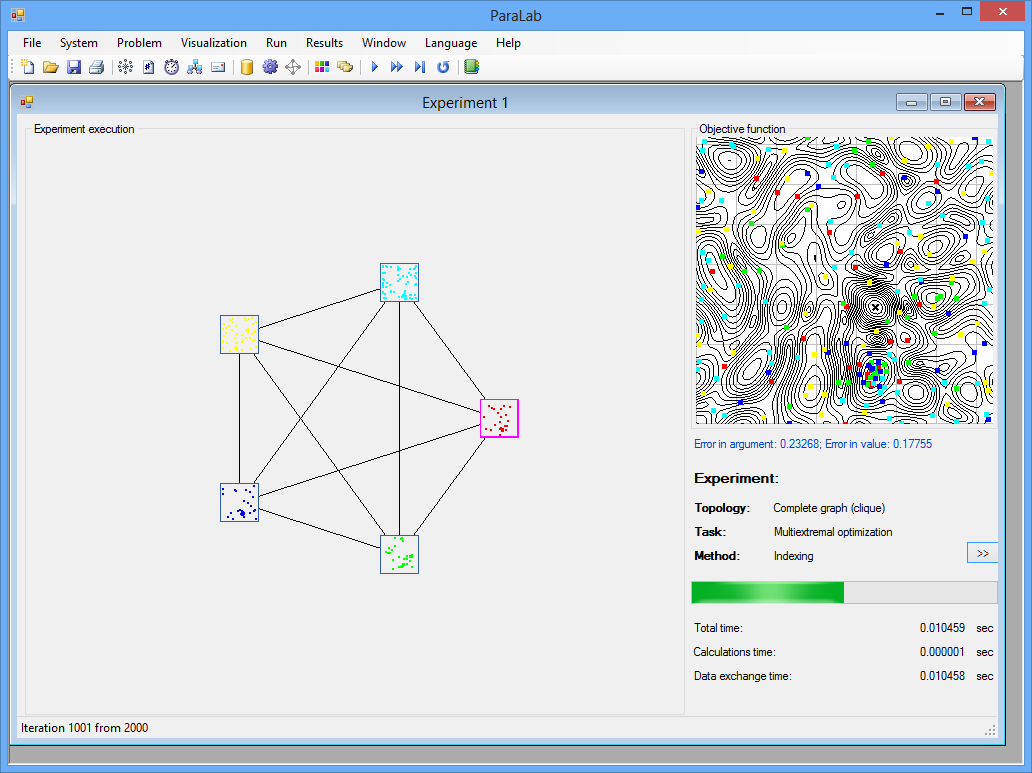
\includegraphics[width=1.0\linewidth]{figures/7_2.png}
\caption{ParaLab main system (global optimization problem is selected)}
\label{7_fig_2}     
\end{figure}

The possibility to choose the method of carrying out the experiments is one of the most important features of ParaLab. The experiments could be performed \textit{in the simulation mode}, i.e., performed on a single processor without using any parallel specialized software like the message transfer libraries. Besides, ParaLab provides the possibility to carry out \textit{the real computational experiments on parallel computers}.

In visualizing the dependencies of the time characteristics on the parameters of the problem and of the computational system for the experiments carried out in the simulation mode the theoretical estimates are used according to the available models of the parallel computations. For the real computational experiments on the multiprocessor computer systems, the dependencies are visualized according to the results of the real numerical experiments. 

It is worth noting that ParaLab provides storing the results of the executed experiments in a special memory buffer. The stored results allow performing the analysis of the obtained data. Any experiment executed earlier can be restored to be recomputed again or to continue the computations according to pre-stored information. 

The education and research processes realized in this way allow getting acquainted with the theoretical basis and assist to develop the methods of design of the parallel algorithms aimed at solving time-consuming applied problems. More detailed information on the ParaLab system is presented in \cite{7_Gergel2010}.


\section{The software system GlobalExpert for parallel solving the global optimization problems}

GlobalExpert is an integrated software for solving the global optimization problems using the parallel computational architectures. This system has been developed on the base of the information-statistical theory of multiextremal optimization in the framework of which many efficient parallel global search algorithms have been designed [ ].

Using GlobalExpert, the researchers can formulate the statement of the optimization problem, select an optimization algorithm from the list of the global search methods build-in in the system, set up the graphic indicators for monitoring the global search process, to execute the computations, obtain and analyze the results. 

GlobalExpert is oriented to the application by the engineers and researchers as an efficient tool for solving the multidimensional global optimization problems. 
A considerable time of the computation of the optimized function at single point, which may reach tens of seconds is a key characteristic of the applied problems. In this case to solve optimization problems in a reasonable time GlobalExpert accumulates and analyzes scrupulously all optimization data computed in the search process. 

The system consists of two main parts: the optimization subsystem and the management one. The management subsystem is implemented as a .NET application using the managed C++ programming language. It is designed for the control of the computations and for displaying the calculated results. Using the management subsystem, the researchers get the following possibilities:

\begin{itemize}
\item \textit{to form an optimization problem} (to define the functions, to select the criteria and constraints, to define the feasible domain for the variables);

\item \textit{to perform a preliminary investigation of the problem} (to plot the function sections and/or the level lines of the problem functions, to analyze the feasible domain of the problem fixing some variables);

\item \textit{to select the optimization method} and to set its parameters;

\item \textit{to select the running mode for the executive module} (serial, parallel on a single computer, parallel in a multiprocessor system);

\item \textit{to monitor the search process in real time};

\item \textit{to modify the problem statement and/or the method parameters} and to solve the problem in a new statement using the search information accumulated earlier.
\end{itemize}

A screenshot of the main window of the management subsystem is presented in Fig.~\ref{7_fig_3}).

\begin{figure}[t]
%\sidecaption[t]
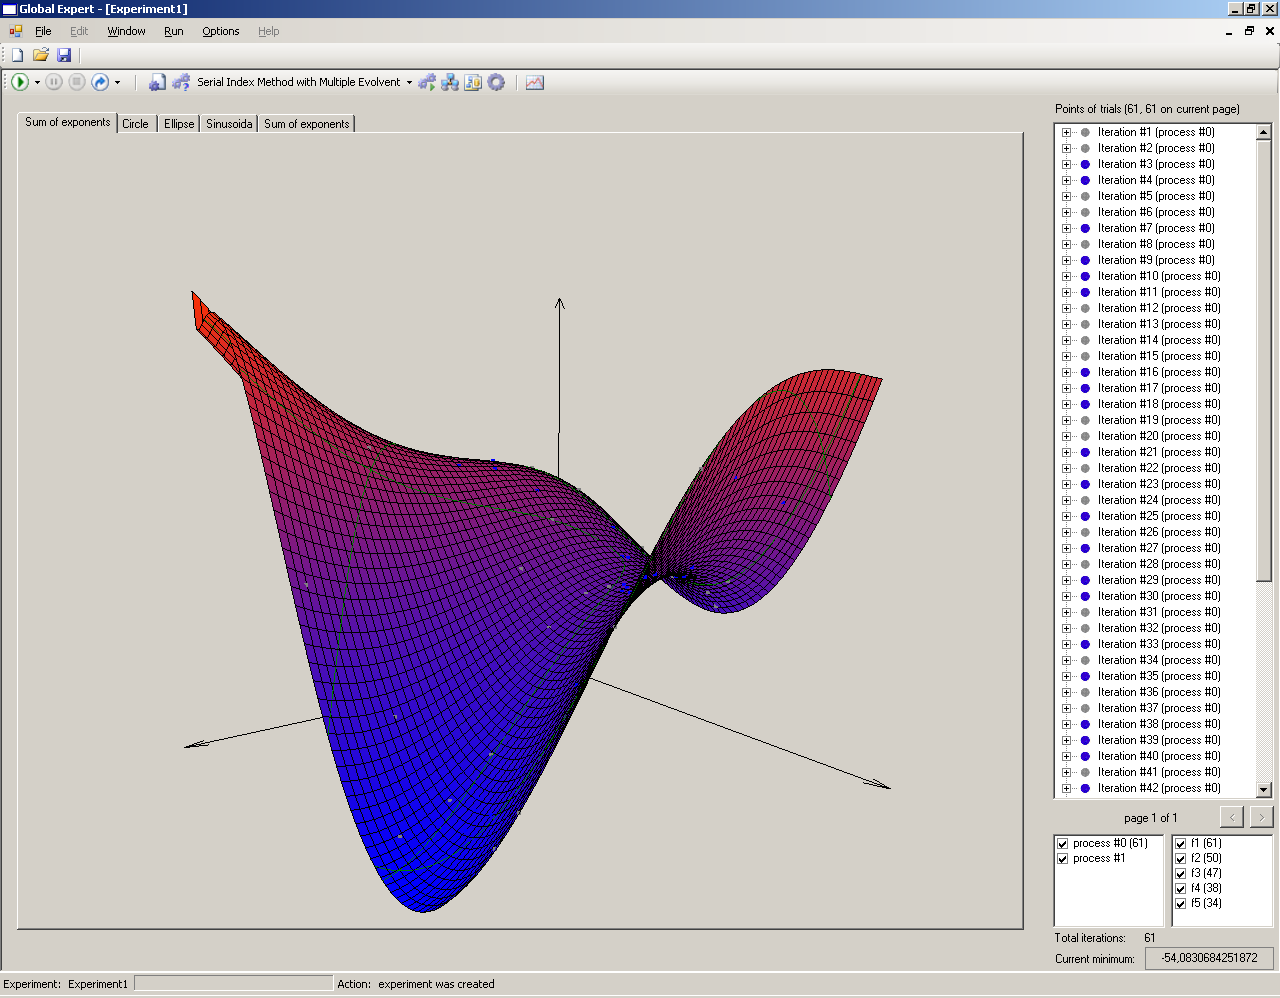
\includegraphics[width=1.0\linewidth]{figures/7_3.png}
\caption{Modeling of the wheel profile}
\label{7_fig_3}     
\end{figure}

The optimization subsystem is implemented in the form of an executable file as well as a module of a dynamic library (developed using С++ programming). In the form of the dynamic library module it can be linked to an application software system as a «solver» for the optimization problems. In the form of the executable file this module can be run either independently (the results are displayed in the console window) or under control of the management subsystem (the results are transferred to the management subsystem for visualizing and processing). 

When performing a large amount of computations the following procedure is recommended for solving time consuming optimization problems. First, one has to perform a preliminary calculations using the management subsystem, to ensure the correct problem statement and correctness of the results obtained when running the problem on a single computer or on a parallel computer with several processors. To run the computations on a real multiprocessor high-performance system, one has to run the executable file of GlobalExpert via the job management of the computational system. With this purpose, the generation of the command line with all options required for running a job on the parallel computer is provided in the management subsystem.

Capacities of the system. GlobalExpert is an integrated program environment for solving the global optimization problems. It allows: 

\begin{itemize}
\item \textit{to modify the statement of the problem} being solved without the loss of the accumulated search information (modification of the constraints set, change of the minimized function, expanding/reducing the search domain);

\item \textit{to use a number of the information global search algorithms} (GlobalExpert includes several serial and parallel algorithms, which demonstrated the high efficiency performance in various applications);

\item \textit{to display the visual information} on the problem being solved in the user-friendly form. The researcher can plot various sections of the problem functions, display the level lines of the minimized functions, the distribution of the iteration points on the function graphs and/or on the level lines, select the iteration points from different processors, etc. 

\item \textit{to accumulate and analyze the results} of the executed experiments. GlobalExpert provides logging of the executed experiments for storing the optimization results. The results of the computations include the search data from all processors, which the system has been run on. The accumulated data are presented in the tabular form, which is convenient for analysis and further processing. 
\end{itemize}



\section{Optimization of the rail transport wheel profile}

The considered problem of the search for the optimum profile of the wheels for the rail transport (railway, subway, tram, etc.) has been solved in the framework of joint research project supported by Russian Foundation for Basic Research (project number 04-01-89002-NVO\_a) and NWO (Netherlands Organization for Scientific Research, project number 047.016.014)  ``Fast Computing in Global Optimization: Sequential and Parallel Environments'', carried out at Lobachevsky State University of Nizhni Novgorod and Delft University of Technology, the Netherlands (TU Delft).

\subsection{Problem Statement}

The problem of the rail transport wheel profile optimization is described in details in \cite{8_Markine2005,8_Markine2007}. Here, a brief description of this problem is presented only. Since the wheels are of the conical shape, the center of a mounted axle is moving along a sinusoid. This process is illustrated in Fig.~\ref{8_fig_1}). The parameters of the contact between the wheel and the rail, such as the radius of rotation, the contact angle, and the angle of inclination for the mounted axle are varied at the transverse displacement of the mounted axle relative to the rail. The relationship between these variations and the transverse position of the mounted axle is determined by the wheel and rail profiles.

\begin{figure}[t]
%\sidecaption[t]
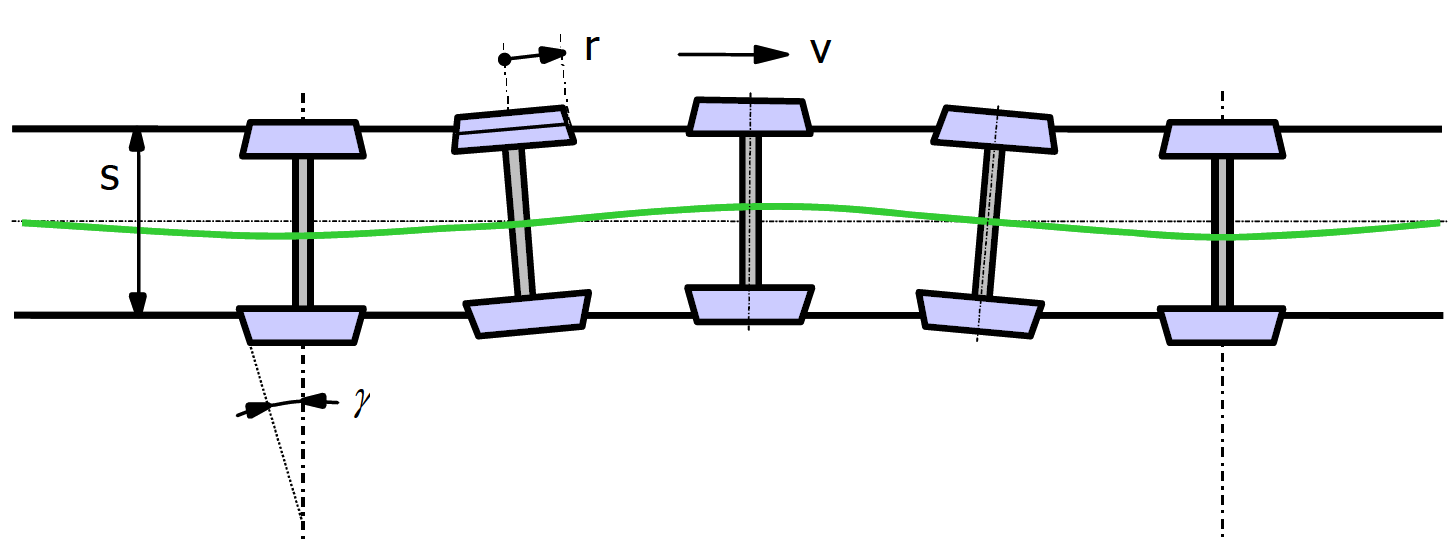
\includegraphics[width=0.9\linewidth]{figures/8_1.png}
\caption{The displacement of the mounted axle}
\label{8_fig_1}     
\end{figure}

The radius of rotation of the wheel at the contact point is an important parameter of the contact between the wheel and the rail. Actually, the radius can be different for the right and the left wheels since the mounted axle can shift relative to the rail (the radii $r_1$ and $r_2$, respectively in Fig.~\ref{8_fig_2}).

\begin{figure}[t]
%\sidecaption[t]
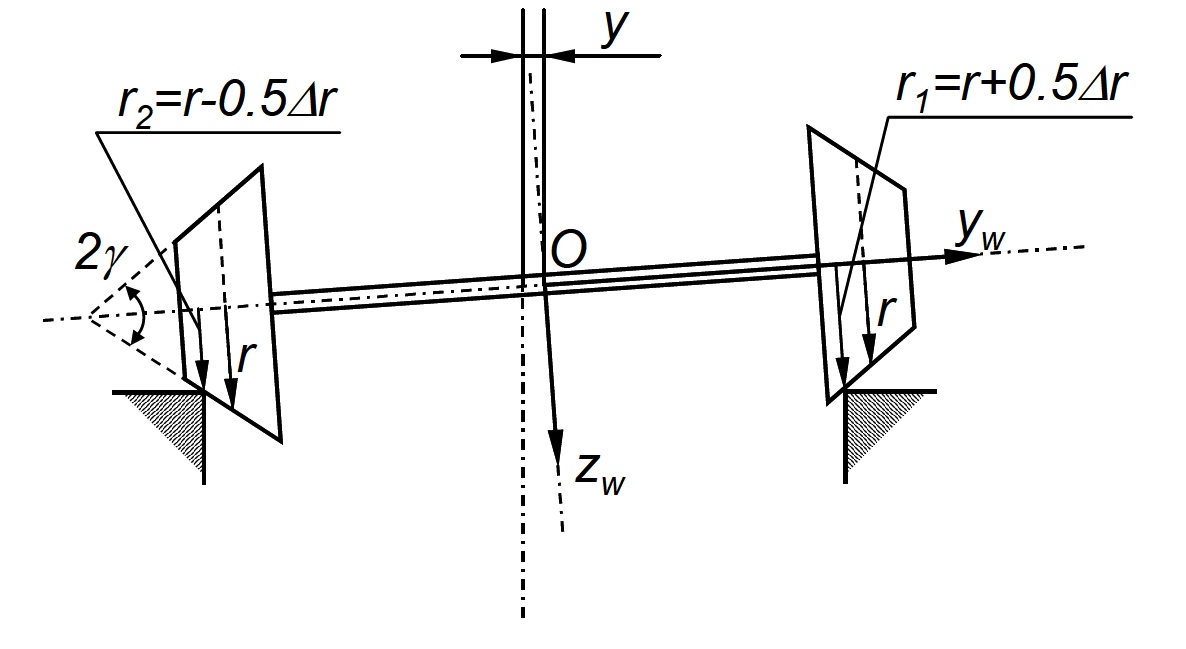
\includegraphics[width=0.7\linewidth]{figures/8_2.png}
\caption{The difference in the radii of rotation}
\label{8_fig_2}     
\end{figure}

When the mounted axle is in the central position, the radii of rotation are the same for the left and right wheels, i.e., $r_1=r_2=r$. The difference in the radii of rotation for the left and right wheels can be defined as a function of the transverse displacement of the mounted axle relative to its central position $\Delta r(x)=r_1(x)-r_2(x)$.

The mathematical model for this problem developed in Technical University Delft consists in the following. The wheel profile is described by B-spline, for building of which a set of points on the edge, on the edge base, and on the rolling surface of the wheel were selected (Fig.~\ref{8_fig_3})). Positions of these points can be varied for the purpose of variation of the profile. In order to reduce the computational costs for the optimization, the positions of the points on the upper surface of the edge as well as on the conical part of the profile were fixed since these parts of the wheel profile do not contact the rails.

\begin{figure}[t]
%\sidecaption[t]
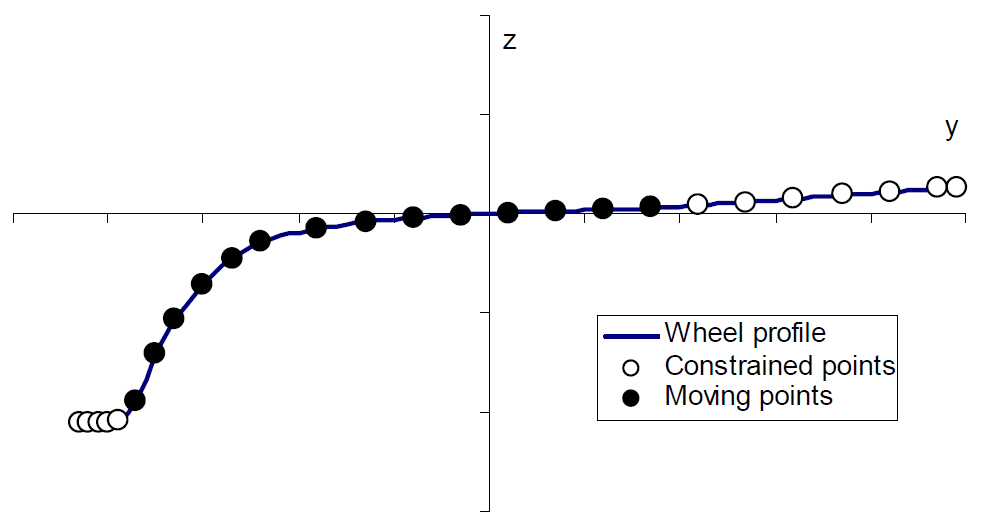
\includegraphics[width=0.7\linewidth]{figures/8_3.png}
\caption{Modeling of the wheel profile}
\label{8_fig_3}     
\end{figure}

The ordinates of the movable points of the spline $z_i$ were selected as the components of the vector of the optimization problem parameters $y$, i.e.,
\[
y=(z_1,...,z_N),
\]
and the abscissas of these points were fixed.

The number of the movable points and, consequently, the number $N$ of variables in the considered problem was equal to $11$. For each parameter   the interval $\left[–1, 1\right]$ was taken as the domain of its variation. The difference of the radii of rotation $\Delta r(x)$ was minimized. The constraints were introduced according to the stability considerations. For example, one of the constraints was imposed on the maximum angle of inclination for the mounted axle.

\subsection{The results of the experiments}

Thus, the optimization problem has $N=11$ parameters and $m=6$ constraints. The objective function as well as the constraint functions is the multiextremal ones. A one-dimensional section of the objective function is presented in Fig.~\ref{8_fig_4} for illustration.

\begin{figure}[t]
%\sidecaption[t]
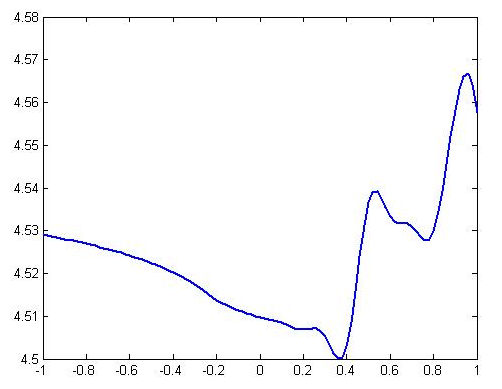
\includegraphics[width=0.7\linewidth]{figures/8_4.png}
\caption{A section of the objective function }
\label{8_fig_4}     
\end{figure}

The constraints have no analytical form and defined by a MATLAB computational procedures. The computation of the values of all problem functions (objective function and constraints) at one point $y$ using Pentium IV processor with the clock frequency of 3 GHz takes about 10 sec. 

Thus, having formulated the problem, let us try to estimate the resources required for its solving in dependence on the method selected. Let us take, for example, the method of full scanning a uniform grid. Having selected 10 variants for the values of each parameter (remind, that the total number of parameters equals to 11), we obtain $10^{11}$ computations at the grid nodes that requires $\sim 10^{12}$ sec., i.e., $\sim 3$ years of computations using a supercomputer with 10 000 processors. Thus, the problem is so hard to solve that the parallel computations are not only necessary but should be supplied with the efficient numerical methods to obtain the results in a reasonable time unavoidably.

The problem described above has been solved by the authors using the parallel index method with the multiple shifted evolvents on a cluster of 4 computers in Delft University of Technology. The search precision in the coordinates was $2^{-10}$ , i.e., 1024 points of each parameter value in the case of the full scanning method. The search time for the optimum estimate was 27 hours. The problem functions values have been computed $4297 + 4415 + 4236 + 4266 = 17214$ times.

The computations carried out at TU Delft for a wheel of the optimum profile demonstrated its service life to increase up to 120 000 km between the profile corrections (more than five times longer as compared to the wheels of the original profile) and the maximum permitted speed to increase from 40 up to 60 m/sec.

\section{Solving the inverse problem of chemical kinetics}

In the present section the results of joint research project carried out at Lobachevsky State University of Nizhni Novgorod and at Institute of Petrochemistry and Catalysis, Russian Academy of Sciences (IPC RAS) \cite{8_Gubaidullin2011}.

\subsection{Problem statement}

The building of the mathematical models of the complex chemical reactions implies the presence of the unknown kinetic parameters (the rate constants, the activation energies, and the frequencies of collisions between the reacting molecules), which could be found by solving the problem of the minimization of the deviations between the calculated data (\textit{the direct problem}) and the experimental ones. Thus, a problem of identifying the mathematical model (\textit{the inverse problem of chemical kinetics}) arises, which in general case is a global optimization problem.

Many problems of physics chemistry imply a considerable amount of computations, nevertheless, providing rather low precision. Investigating the inverse problems of chemical kinetics requires solving many systems of differential and algebraic equations. The kinetics of complex chemical reactions is featured by the presence of parameters varying fast and slowly (because various stages of reactions go with different rates). Therefore, solving the direct kinetic problems is complicated by the hardness of the differential equations describing the mechanisms of these reactions.

The direct kinetic problem for the isothermal non-stationary model in a closed system is Cauchy problem for a system of ordinary differential equations
\begin{equation} 
 \frac{dx_i}{dt}= F_i, i=1,..,M; \; F_i=\sum_{j=1}^{N}{S_{ij}w_j}
\end{equation}
\begin{equation} 
 w_j=k_j\prod_{i=1}^{M}{\left(x_i\right)^{\left|\alpha_{ij}\right|}}-k_{-j}\prod_{i=1}^{M}{\left(x_i\right)^{\left|\beta_{ij}\right|}}
\end{equation}
with the initial conditions $t=0$, $x_i(0)=x_i^0$, where 
\begin{itemize}
	\item $x_i$ are the concentrations of the substances (\textit{the molar fractions}) participating in the reaction;
	\item $M$ is the number of substances; 
	\item $N$ is the number of steps;
	\item $S_{ij}$ are the stoichiometric matrix; 
	\item $w_j$ are the rates of the $j$-th step, $1/{hr}$; 
	\item $k_j$, $k_{-j}$ are the reduced rate constants for the forward and reverse reactions ($1/{hr}$), respectively;
	\item $\alpha_{ij}$ are the negative elements of $S_{ij}$, and $\beta_{ij}$ are the positive elements of $S_{ij}$.
\end{itemize}

Since a part of the constants $k_j$, $k_{-j}$, as a rule, are not known, the problem of identification of the mathematical model of  the inverse kinetic problem arises. This problem is a minimization one for the function of the deviation between the calculated data and the experimental ones
\begin{equation} \label{8_chem_func}
F=\sum_{i=1}^n{\sum_{j=1}^M{\left|x_{ij}^p-x_{ij}^{\epsilon}\right|}}\rightarrow \min,
\end{equation}
where
\begin{itemize}
	\item $x_{ij}^p$ are the calculated values of the observable substances concentrations  (\textit{molar fractions});	
	\item $x_{ij}^{\epsilon}$ are the values of the observable substances concentrations measured experimentally (\textit{molar fractions});
	\item $n$ is the number of the experimental points.
\end{itemize}

To find the activation energies and the collision frequencies of the molecules reacting at the elementary step, Arrhenius equation
\[
k=Ae^{-\frac{Ea}{RT}}
\]
is used, where
\begin{itemize}
	\item $k$ is the reduced rate constant for the elementary step, $1/hr$;	
	\item $E$ is the activation energy, $J/{mol}$;
	\item $R$ is gas constant, $J/{(mol \cdot K)}$;
	\item $А$ is the collision frequency for the reacting molecules;
	\item $T$ is the temperature, $K$.	
\end{itemize}

Since in the search for the rate constants of the elementary steps, these ones may fall into the area, where the differential equations system describing the reactions may appear to be a stiff one, Mishelsen method with automatic step selection is applied to solving the direct problem \cite{8_Gubaidullin2010}. As the model output data $x_{ij}^p$ depend on the values of the constants $k_j$, $k_{-j}$ nonlinearly, problem (\ref{8_chem_func}) is a multiextremal optimization problem.

\subsection{The results of the experiments}

Traditionally, the methods based on the random search ideas had been applied in IPC RAS for solving problem (\ref{8_chem_func}). The typical computation costs were several days of continuous computations. Within the framework of the joint research project by IPC RAS and Lobachevsky State University of Nizhni Novgorod it was proposed to apply the efficient parallel global optimization methods developed in UNN. 

For the application of the novel identification technique the mathematical model for the reaction of the catalytical carboalumination of olefins and acetylenes with the assistance of threealkylalanes in the presence of transition metal complexes was selected. This reaction has applied in the laboratory research at IPC RAS as an efficient method for the synthesis of new Me-C (methyl-carbon), Et-C (ethyl-carbon), and C-C (carbon-carbon) bonds \cite{8_Parfenova2009}. The natural experiments of conducting the reactions of the catalytical carboalumination of olefins and acetylenes for different temperatures and fixed initial concentrations have been carried out in IPC RAS. In the experiments, the concentrations of five substances were traced and their percentage ratios were determined. A number of schemes for the mathematical description of the reaction of catalytical carboalumination of olefins and acetylenes (including the parameters to be identified) have been proposed in IPC RAS. As a priority problem of the identification of the unknown parameters, it was required to determine the rate constants for the elementary steps for the proposed reaction schemes for various temperatures as well as to find the activation energies for the elementary steps for various catalysts. These schemes and the identification problem have been described in details in \cite{8_Gubaidullin2011}. Here, note that the minimization problem arising depends on 10 parameters and is box-constrained one. The computational costs for the function value at one point are $\sim 3$ sec. (Intel Xeon 3.2 GHz). The objective function is  multiextremal that is confirmed by its two-dimensional section presented in Fig.~\ref{8_fig_5}. 

\begin{figure}[t]
%\sidecaption[t]
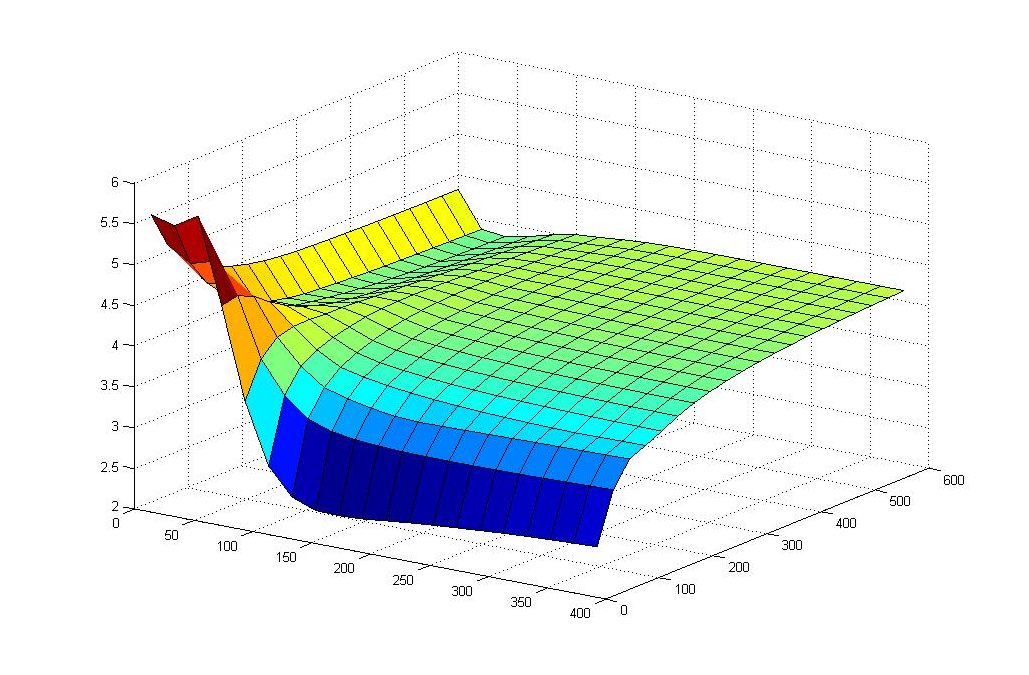
\includegraphics[width=0.8\linewidth]{figures/8_5.png}
\caption{Two-dimensional section of the objective function}
\label{8_fig_5}     
\end{figure}

As a result of the computations, the estimates of the rate constants for the elementary steps for the 10- and 12-step reactions schemes of the carboalumination in the presence of $Cp_2 ZrCl_2$ catalyst have been obtained. The objective function value at the obtained optimizer was $F = 3.040$. It appeared to be impossible to achieve the function value close to zero because the experimental data contains the uncertainties. Nevertheless, the model identified using the parallel global optimization method allowed obtaining a good conformity between the calculated data and the experimental ones. As an illustration, the comparison of the computed and experimental concentrations of substances participating in the reactions is presented in Fig.~\ref{8_fig_6}.

\begin{figure}
\begin{minipage}{0.5\linewidth}
\center{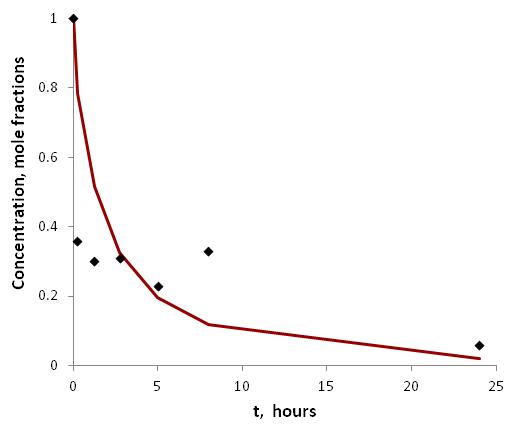
\includegraphics[width=1.0\linewidth]{figures/8_6a.png} \\ (a)}
\end{minipage}
\hfill
\begin{minipage}{0.5\linewidth}
\center{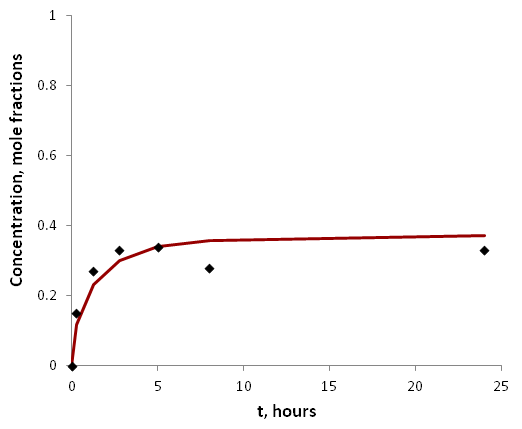
\includegraphics[width=1.0\linewidth]{figures/8_6b.png} \\ (b)}
\end{minipage}
\caption{The comparison of the calculated data with the experimental ones}
\label{8_fig_6}
\end{figure}


\section{Identification of the dynamic balance normative models of the regional economy}

In the present section, the results obtained within the research project supported by RFBR ``Parallel global optimization methods in the identification of the dynamic balance for the normative models of the regional economy'', project 11-07-97017, carried out jointly by the research teams from Lobachevsky State University of Nizhni Novgorod and from Dorodnicyn Computing Centre of RAS are presented \cite{8_Gergel2011}.

\subsection{Problem statement}

The regional economy (the district, region, or state, etc. level) was the object of investigations. For the mathematical description of the economical processes taking place at the regional level, a dynamic balance normative economic model has been proposed in Dorodnicyn Computing Centre of RAS \cite{8_Olenev1999}. This model is a general one. However, it includes a significant number of parameters  being specific to the different regions. It is possible to find these parameters (or \textit{to identify the model}) by solving the problem of minimization of the deviation of the calculated time series of the macroeconomic measures from the corresponding historic statistical data. The functions entering the problem statement are the nonlinear ones. As a result, the problem of identification of the mathematical economic model is the global optimization one.

Once the model was identified, it could be applied to verify various possible scenarios of the regional economic development on the base of the experiments with the model. The conclusions and predictions obtained using the identified mathematical model, in principle, could be disposed experimentally. This enables to correct further the model in order to obtain more justified prognosis based on the model being improved continuously. 

The problem of the identification of the multisector model of the regional economy presented here has been solved on the base of the data available for Nizhni Novgorod region, Russia. As it has been already mentioned above, the normative models include a large number of unknown parameters (the normatives of the distribution of the products and the normatives of distribution of the financial resources). In order to identify these parameters, it was proposed to apply the efficient parallel global optimization methods. The application of these algorithms on the supercomputer systems allows increasing the level of complexity of the mathematical models of the regional economy expressed by the number of the independent parameters. Carrying out the scenario computations based on the identified models of the regional economy allows more exact prognosis of the economic consequences of various strategic decisions.

\subsection{The description of the model of the regional economy}

The economy of Nizhni Novgorod region can be aggregated into three main sectors with approximately equal power:
\begin{itemize}
	\item the branches of the infrastructure, production and distribution of raw materials (agriculture, electric power industry, development, transportation, state administration, education, public health);
	\item the manufacturing branches (machine building and metal working, chemical and petrochemical industry, fuel industry, ferrous and nonferrous metallurgy, construction materials industry, timber, woodworking, and pulp-and-paper industry, consumer goods industry, food, pharmaceutical, chemical, microbiological industry, flour-and-cereals and feed mill industry, printing industry, scientific complex);
	\item the service branches (trading, operations with real estate, financial services, other services).
\end{itemize}

Let us select the following economic agents while designing the model: Regional Government, the producers represented by the three sectors selected above, the banking system, and the households of the region, the external vendors and consumers.

In spite of absence of rich natural resources in Nizhni Novgorod Region its economy is one of the most developed one with respect to the industry among the regions of Russian Federation. The processing branches of industry, a powerful military industrial complex, well-developed fundamental scientific complex are the base of the industry in Nizhni Novgorod Region and there are good prospects for the development of the high-tech industries and of the innovative branches.

The three-sector variant of the general balance model with supplies of products, factors of production, and financial resources in taxation and the illegal circulation of goods and finances \cite{8_Olenev2007} has been applied as the base for the design of the mathematical model of the regional economy. Remind that the producers in the model of Nizhni Novgorod Region economy are represented by three sectors: 
\begin{itemize}
	\item the infrastructure complex ($X$),
	\item the manufacturing branches complex ($Y$),
	\item the services, mortgage, financial, and trading branches complex ($Z$).
\end{itemize}
The producers (the sectors of the regional economy $X$, $Y$, $Z$) use labor, capital, and the intermediate production of the partner sectors. The producers deliver their products to the internal markets and to the external ones. The households $L$ offer the labor and consume the final products. The resellers $T$ redistribute the goods and financial flows. The banking system $B$ lends money to the producers with the purpose to receive the banking profit. Regional Government $G$ collects the taxes from the producers and the households and manages the budget expenditures. Each market is assumed to establish its own prices for each kind of products. The variations of the prices are assumed to be inversely proportional to the variation of the supplies of the corresponding products. 

In order to account for the illegal circulation of the goods and money, the producers were assumed to divide the manufactured products into the legal part and the illegal one. The latter does not undergo the taxation. As a result, the producers receive two kinds of income: the ``legal'' and the ``illegal'' one. The ``illegal'' money can be laundered and the reserves undergo penalties.

All the consumers’ money is assumed to be legal. The consumers’ income is assumed to be distributed between the acquisition of the legal products and the illegal ones from all sectors according to the predefined percentages. The production sectors $m = X,\;Y,\;Z$ pay the profit tax $n_1$, the value added tax $n_2$, the excise tax on the total output $n_3^m$ , the unified social tax on the payroll $n_4$, and the exports customs duties $n_5$. The households $L$ within the framework of the model pay the import customs duties $n_6$ and the income tax on the wages $n_7$.

The criteria and the parameters of the model have the upper and lower indices. The upper indices are used for the agents and the lower ones for the valuables. The supplies of each valuable are distributed according to the normative  $a_i^{nm}$, which are the portions of the amount of the valuable $i$ being transferred from the agent $n$ to the agent $m$. The distribution of money is also performed according to some normative $b_i^{nm}$, which are the portions of the money resources of the agent $m$ transferred to the agent $n$ for the product $i$. The capital coefficients are also defined by the normatives $c_i^m$ , which are the normalized amount of the product $i$ spent for the producing a unit of a fund product for the agent $m$.

The identification of the parameters was performed by the comparison of the output time series of the model variables with the available statistical time series in 2000--2008. As a criterion of proximity of the calculated time series to the statistical ones, Theil index was applied, which has been calculated according to the formula
\[
U=\frac{\sqrt{\sum{(x_i-y_i)^2}}}{\sqrt{\sum{x_i^2}}+\sqrt{\sum{y_i^2}}}
\]
The close the index to zero, the close the series compared.

\subsection{The results of the experiments}

The detailed description of the designed model is beyond the scope of this paper. The additional information can be found in \cite{8_Gergel2011}. Here we note that the global optimization problem arising in the model identification process has $60$ independent parameters, $86$ nonlinear constraints, and a multiextremal objective function. As an illustration, a two-dimensional section of the objective function confirming its essential multiextremality is presented in Fig.~\ref{8_fig_7}. 

\begin{figure}[t]
%\sidecaption[t]
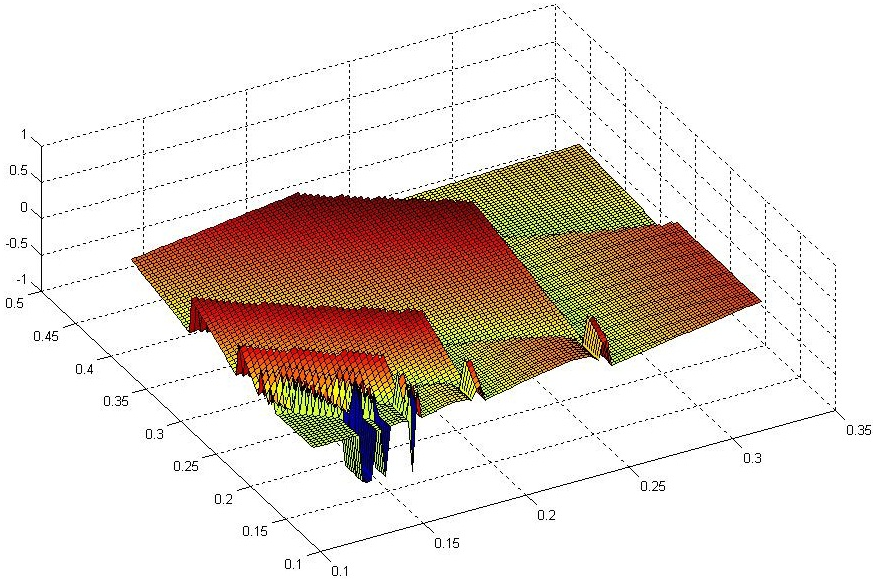
\includegraphics[width=0.8\linewidth]{figures/8_7.png}
\caption{Two-dimensional section of the objective function}
\label{8_fig_7}     
\end{figure}

This problem has been solved on the cluster of Lobachevsky State University of Nizhni Novgorod using the parallel index method with the rotated evolvents (8 processors were employed). The estimate of optimum was obtained after $300 000$ iterations, the computation time of obtaining an estimate was $26$ minutes. Total computation time was $3$ hours.

Using the identified mathematical model of Nizhni Novgorod Region, the scenario computations reflecting the dynamics of the economic indicators of the region for various economic policies (the pessimistic scenario, the basic, and the optimistic one) have been carried out in Computing Centre of RAS.

\begin{thebibliography}{99.}

\bibitem{7_Gergel1993} 
Gergel, V.P.: A software system for multiextremal optimization. European Journal of Operational Research. \textbf{65(3)}, 305--313 (1993)

\bibitem{7_Pinter1996}
Pintér, J.D.: Global Optimization in Action (Continuous and Lipschitz Optimization: Algorithms, Implementations and Applications). Dordrecht: Kluwer Academic Publishers (1996)

\bibitem{7_Gergel2010}
Gergel, V.P., Labutina, A.A.: The ParaLab system for investigating the parallel algorithms. Lecture Notes in Computer Science. \textbf{6083}, 95--104 (2010)

\bibitem{8_Markine2005} 
Shevtsov, I.Y., Markine, V.L., Esveld, C.: Optimal design of wheel profile for railway vehicles. Wear. \textbf{258(7-8)}, 1022--1030 (2005)

\bibitem{8_Markine2007} 
Shevtsov, I.Y., Markine, V.L., Esveld, C.: An inverse shape design method for railway wheel profiles. Structural and Multidisciplinary Optimization. \textbf{33(3)}, 243--253 (2007)

\bibitem{8_Gubaidullin2011}
Gubaidullin, I.M., Ryabov, V.V., Tikhonova, M.V.: Application of the global optimization index method to solving inverse problems of chemical kinetics. Numerical methods and programming. \textbf{12(1)}, 137--145 (2011) (in Russian)

\bibitem{8_Gubaidullin2010}
Tikhonova, M.V., Gubaidullin, I.M., Spivak, S.I.: The numerical solution of the direct chemical kinetics problem by the Rosenbrock's and Mishelsen's methods for the stiff systems of differential equations. MVMS Journal. \textbf{12(12}, 26--33 (2010) (in Russian)

\bibitem{8_Parfenova2009}
Parfenova, L.V., Gabdrakhmanov, V.Z., Khalilov, L.M., Dzhemilev, U.M.: On study of chemoselectivity of reaction of trialkylalanes with alkenes, catalyzed with $Zr$ $\pi$-complexes. Journal of Organometallic Chemistry. \textbf{694(23)}, 3725--3731 (2009)

\bibitem{8_Gergel2011}
Gergel, V.P., Gorbachev, V.A., Olenev, N.N., Ryabov, V.V., Sidorov, S.V. Parallel global optimization methods for identification of the dynamic balance normative model of regional economy. Bulletin of South Ural State University. \textbf{25(9)}, 4--15 (2011) (In Russian)

\bibitem{8_Olenev1999}
Avtukhovich, E.V., Guriev, S.M., Olenev, N.N., Petrov, A.A., Pospelov, I.G., Shananin, A.A., Chukanov, S.V.: A Mathematical Model of the Transition Economy. The Computing Centre of the Russian Academy of Sciences, Moscow (1999) (In Russian)

\bibitem{8_Olenev2007}
Olenev, N.N.: Model of innovation potential of regional economy. Proceedings of international conference ``Economy of depressed areas: problems and prospects of progress of regional economy''. Altai State University Press. 178--188 (2007) (In Russian)

\end{thebibliography}

%\end{document}
